\subsection{Primeras simulaciones}

El objetivo de esta sección es analizar la influencia del potencial de Pauli \eqref{eq:def_int_pauli} en la simulación de NM. 
Como dijimos, el potencial nuclear de QCNM \eqref{eq:pot_QCNM} no distingue entre protones y neutrones, por lo que a efectos de ese potencial tenemos $N=N_n+N_p$ partículas idénticas.
Con la introducción del potencial de Pauli, separaremos las $N=1000$ partículas según sus componentes de spin e isospin, por lo que $N = N_n^\uparrow+N_n^\downarrow+N_p^\uparrow+N_p^\downarrow$.
En particular, nos interesa un caso simétrico, tomamos $N_n^\uparrow=N_n^\downarrow=N_p^\uparrow=N_p^\downarrow = N/4 = 250\equiv n$.
Dado que la exclusión de Pauli solo puede darse para partículas con la misma componente de spin e isospin, tendremos $N(N-1)/2$ pares de interacción nuclear y $4n(n-1)/2 = N(N/4-1)/2$ 
pares de interacción de Pauli (aproximadamente la mitad). 
Utilizaremos los parámetros de Dorso \eqref{eq:params_dorso} en el potencial de Pauli y una masa $m_n=m_p=938MeV/c^2$.

Las densidades habituales de NM resultan del orden de $0.1$fm$^{-3}$, que para un sistema de $N=1000$ partículas exige cajas de lado $L\sim 20$fm.
Si recordamos que previamente impusimos un $s_{cut}^2=10$ para el potencial se Pauli equivalente a una distancia de $s_{cut}q_o \approx 19$fm, vemos inmediatamente que utilizar un criterio de
mínima imagen resulta inviable al exigir $r_{cut}\leq L/2$; necesitaríamos aumentar la cantidad de partículas a $N\sim8000$ para alcanzar densidades $\rho=0.3$fm$^{-3}$.

Es por esto que decidimos usar las condiciones periódicas del sistema sin el criterio de mínima imagen, permitiendo la interacción simultánea con múltiples imágenes de una misma partícula.
Agregando $l$ copias del sistema en cada una de las direcciones (llamadas \textit{layers}), nos basta que $r_{cut}\leq l.L$ para asegurar que no estamos perdiendo interacciones.
Con el objetivo de tener la menor cantidad de \textit{layers} posibles para minimizar el costo computacional, reducimos la distancia de corte de Pauli a $s_{cut}=6$fm, donde el potencial cae a un $5\%$
del valor máximo $D$.
Dado que el potencial nuclear tiene un 
\[r_{cut}^{(N)} = 6\text{fm}\leq r_{cut}^{(P)} = 14.7\text{fm} \]
 nos basta elegir un $l$ que cumpla $l.L \geq 14.7$fm.
Sin embargo, el valor de $L$ dependerá de $\rho$, por lo que si acotamos $\rho\leq 0.3$fm$^{-3}$ vemos que nos basta tomar $l=1$.
Por lo tanto, una única capa de imágenes bastará para nuestras simulaciones.


\begin{figure}[H]
	\centering
	\subfigure[$\rho=0.005$fm$^{-3}$; ñoquis]{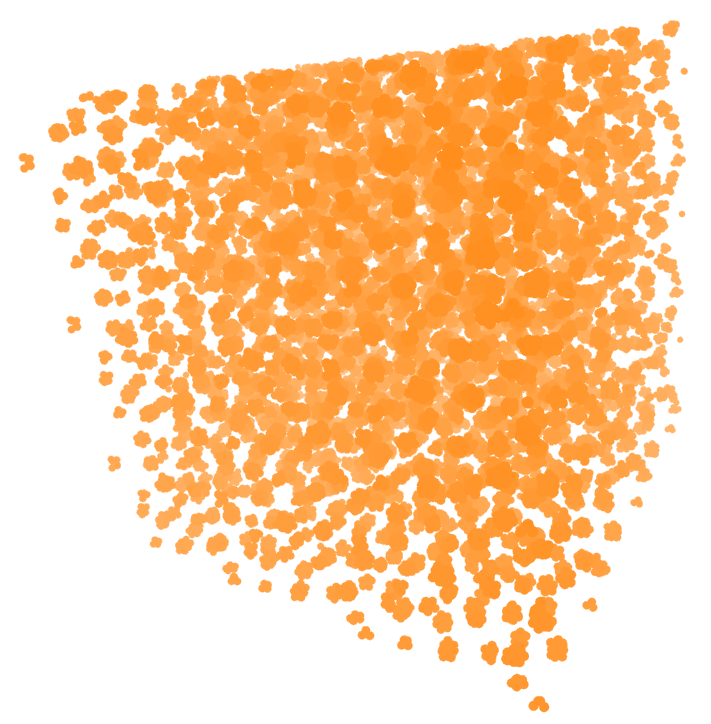
\includegraphics[width=0.3\columnwidth]{NM/pastas_x1/noquis_0,005_x1.png}}
	\hspace{0.03\columnwidth}
	\subfigure[$\rho=0.03$fm$^{-3}$; ñoquis]{
\includegraphics[width=0.3\columnwidth]{NM/pastas_x1/noquis_0,03_x1.png}}
	\hspace{0.03\columnwidth}
	\subfigure[$\rho=0.04$fm$^{-3}$; ñoquis-spaghettis]{
\includegraphics[width=0.3\columnwidth]{NM/pastas_x1/noquis-fideos_0,04_x1.png}}
	\subfigure[$\rho=0.05$fm$^{-3}$; spaghettis]{
\includegraphics[width=0.3\columnwidth]{NM/pastas_x1/fideos_0,05_x1.png}}
	\hspace{0.03\columnwidth}
	\subfigure[$\rho=0.06$fm$^{-3}$; spaghettis-lasagnas]{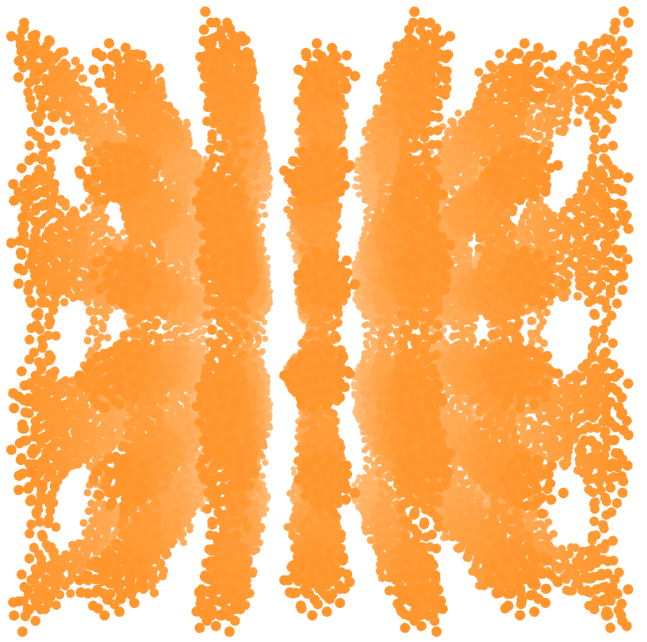
\includegraphics[width=0.3\columnwidth]{NM/pastas_x1/fideos-lasagna_0,06_x1.png}}
	\hspace{0.03\columnwidth}
	\subfigure[$\rho=0.08$fm$^{-3}$; lasagnas]{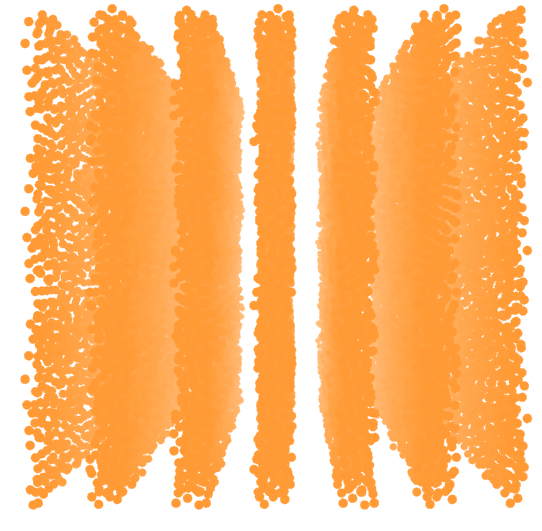
\includegraphics[width=0.3\columnwidth]{NM/pastas_x1/lasagna_0,08_x1.png}}
	\subfigure[$\rho=0.125$fm$^{-3}$; túneles]{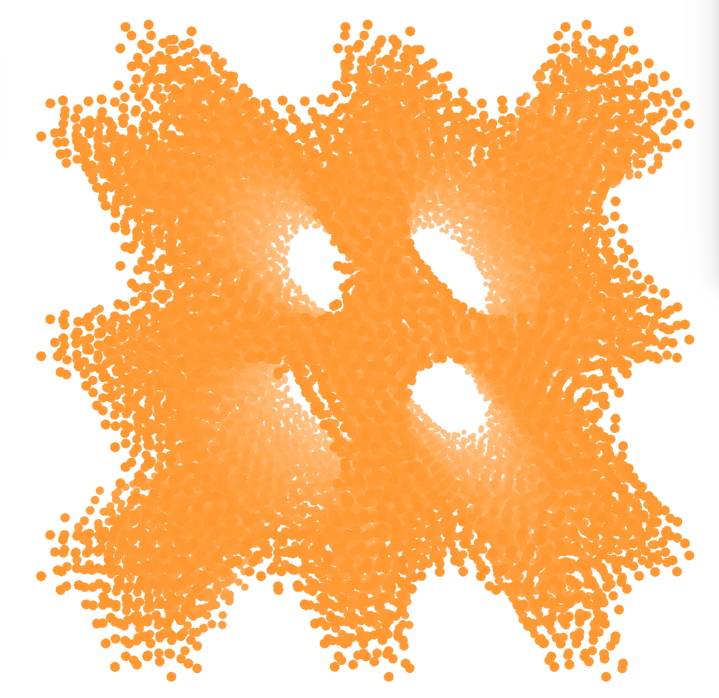
\includegraphics[width=0.3\columnwidth]{NM/pastas_x1/tuneles_0,125_x1.png}}
	\hspace{0.03\columnwidth}
	\subfigure[$\rho=0.16$fm$^{-3}$; burbujas]{
\includegraphics[width=0.3\columnwidth]{NM/pastas_x1/burbuja_0,16_x1.png}}
	\hspace{0.03\columnwidth}
	\subfigure[$\rho=0.175$fm$^{-3}$; gas homogéneo]{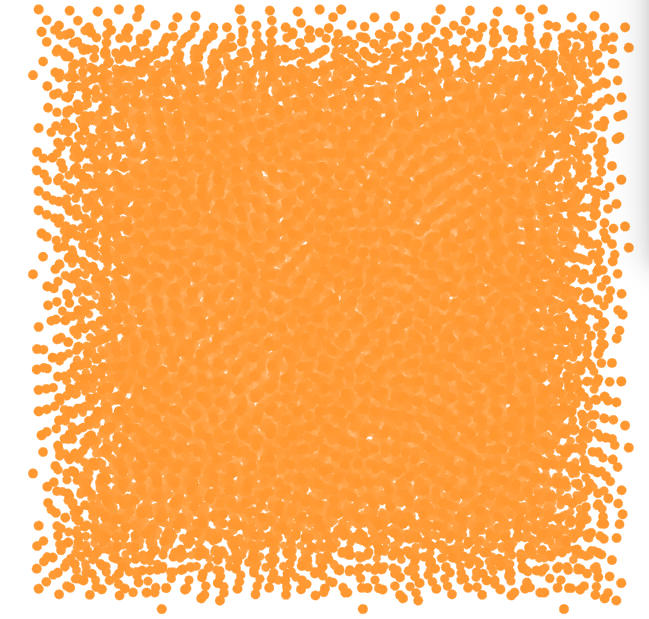
\includegraphics[width=0.3\columnwidth]{NM/pastas_x1/gas_0,175_x1.png}}
	\caption{Distintas topologías halladas durante la simulación.
	También se muestra una layer adicional de imágenes para facilitar visualización.}
	\label{fig:pastas_x1}
\end{figure}

Dado que nos interesa el estado fundamental de NM, hicimos simulaciones de Montecarlo para $T=0.5$MeV, comenzando el sistema como una red simple cúbica con impulsos según la distribución de Boltzmann.
Evolucionamos el sistema para múltiples densidades $\rho$ entre $0.005$fm$^{-3}$ y $0.3$fm$^{-3}$ hasta que la energía se estabilizara, para lo cual bastaron $10^5N$ pasos.

Los resultados de estas simulaciones fueron inesperados.
Para empezar, en la \textbf{Figura \ref{fig:pastas_x1}} podemos ver las configuraciones de algunas densidades seleccionadas.
Estas configuraciones se muestran con la primer capa de imágenes para poder apreciar mejor las pastas resultantes.
En los casos de fideos y lasagnas, podemos ver que tenemos más de una estructura por celda, algo no habitual en NM según lo que discutimos en la sección \ref{sec:intro_NM}.
Además, se muestran configuraciones menos definidas en $\rho=0.04$fm$^{-3}$ y $\rho=0.06$fm$^{-3}$, probablemente densidades muy cercanas a la transición entre pastas.
Para $\rho\geq 0.17$fm$^{-3}$ las pastas desaparecen y dan lugar a un gas uniforme. 

Lo más extraño, sin embargo, es la tendencia de los ñoquis a reducir su tamaño a medida que $\rho$ baja. 
Para $\rho=0.03$fm$^{-3}$ el sistema está compuesto de ñoquis de $\sim 100$ partículas, pero al alcanzar $\rho=0.005$fm$^{-3}$ el tamaño descendió a $\sim 10$ partículas.
Esta tendencia decreciente parecería indicar que en el límite de bajas densidades $\rho\to0$ el estado fundamental del sistema resulta el de ñoquis de menos de $10$ partículas, 
lo cual no es consistente con la existencia de núcleos atómicos. 
En particular, implica que la repulsión dada por el potencial de Pauli supera la atracción del potencial nuclear.
Esta ineficiencia energética de acercar nucleones puede darse por 2 razones; bien Pauli tiene una gran intensidad $D$ o un gran alcance $q_o$. 
El primer caso es obvio, pero el segundo implica que si 2 partículas logran estar muy cerca sus impulsos deben diferir considerablemente, lo cual impone un aumento de la energía cinética.

Más allá de la topología, analizamos la energía por partícula del sistema $E$ en función de $\rho$, esperando encontrar un mínimo en $\rho=0.04$fm$^{-3}$ de $\sim -16$MeV.
En la \textbf{Figura \ref{fig:Evsrho_QCNMx1}} podemos ver que esto no es así, dado que hayamos un mínimo de $\sim -47$MeV en $\rho=0.2$fm$^{-3}$.
Esta energía de ligadura resulta el triple de la esperada y desplaza la densidad de saturación un $\sim 25\%$. 
También se encuentran marcados los distintos regímenes de pasta del sistema. 
Además, podemos apreciar la clara concavidad de la curva, aún cuando esperamos que en el régimen de pastas esta tienda a ser constante (ver sección \ref{sec:intro_NM}).

\begin{figure}[H]
	\centering
	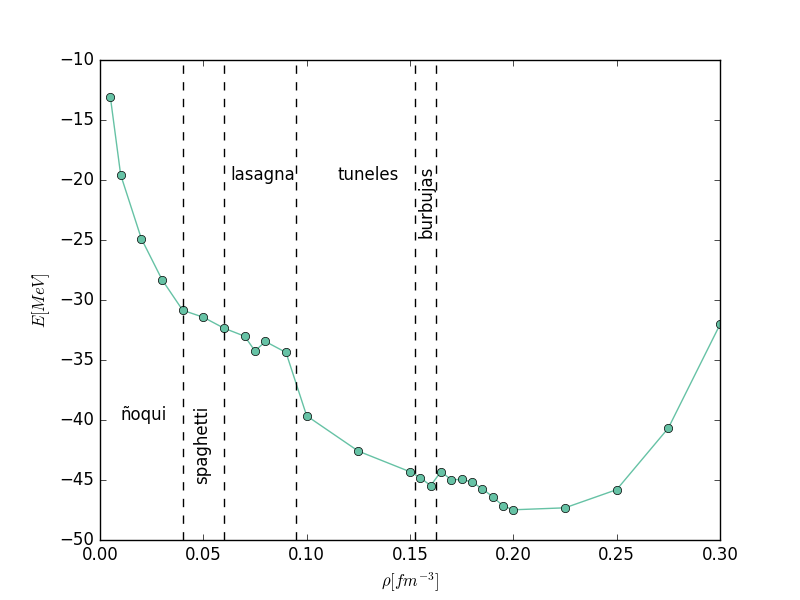
\includegraphics[width=0.9\textwidth]{NM/Evsrho_full_x1.png}
	\caption{Energía por nucleón en función de la densidad $\rho$. 
		La curva es aproximadamente cóncava y presenta pastas en las densidades menores a la saturación $\rho_o=0.16$ fm$^{-3}$. 
		En $\rho=0.2$ fm$^{-3}$ se encuentra el mínimo de $-47$MeV, una fuerte sobrestimación. }
	\label{fig:Evsrho_QCNMx1}
\end{figure}

\subsection{Reajuste de parámetros y enfriamiento}

Frente a la sobrestimación de las energías de ligadura de la \textbf{Figura \ref{fig:Evsrho_QCNMx1}}, la respuesta natural fue buscar reducir esta energía.
Para esto, resultó natural reducir la intensidad $V_o$ del potencial nuclear presentado en \ref{sec:intro_NM} a la mitad.
Con el objetivo adicional de estudiar la formación de estas pastas, inicializamos el sistema en $T=5$MeV y lo enfriamos escalonadamente hasta alcanzar los $T=0.5$MeV.
En cada temperatura, muestreamos la energía por partícula para obtener la curva calórica.
En la \textbf{Figura \ref{fig:EvsT_pastas}} podemos apreciar algunas de estas curvas calóricas para densidades específicas; una para cada una de las pastas halladas.
Estas pastas resultaron con una única estructura por celda para spaghettis y lasagnas, más acorde a lo esperado en NM.

En todos los casos, la pasta se originó alrededor de $T=3.5$MeV donde puede apreciarse una región de inestabilidad en los valores de $E$.
Sin embargo, es ciertamente llamativo que no exista salto en la energía entre el estado fundamental de la pasta en $T=0.5$MeV.
Este salto en la energía está asociado a la cristalización de la pasta, lo cual como discutimos en la sección  \ref{sec:gr_pauli_gas}, no resulta sencillo en presencia del potencial de Pauli.

\begin{figure}[H]
	\centering	%trim={<left> <lower> <right> <upper>}
	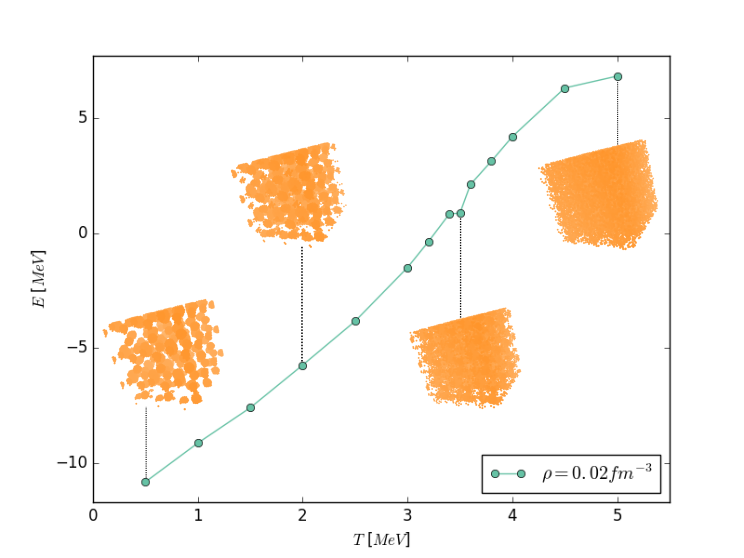
\includegraphics[trim = 5mm 0mm 10mm 5mm, clip, width=0.48\textwidth]{NM/EvsT_noquis.png}
	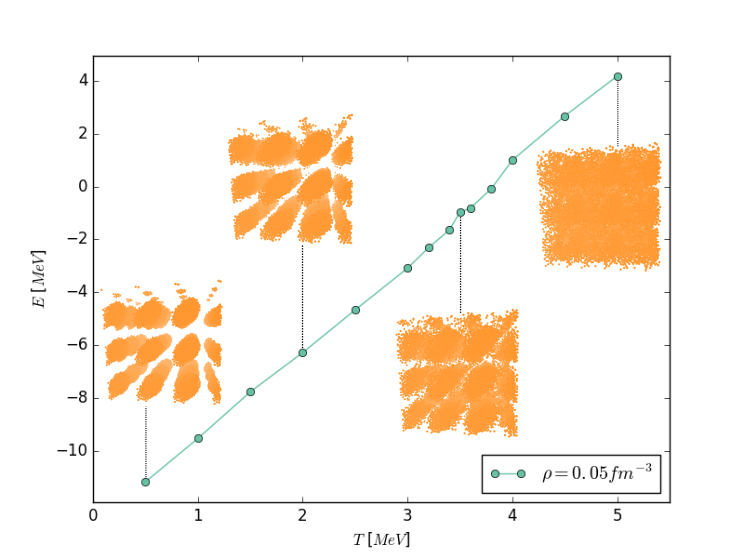
\includegraphics[trim = 5mm 0mm 10mm 5mm, clip, width=0.48\textwidth]{NM/EvsT_fideos.png}
	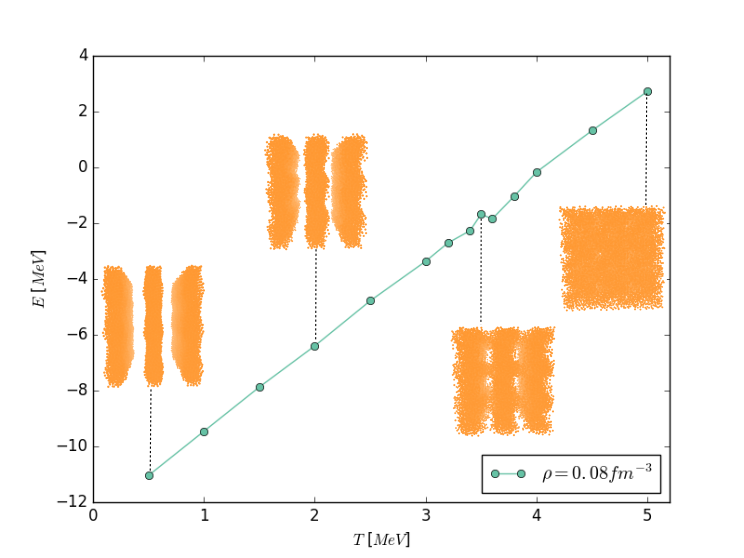
\includegraphics[trim = 5mm 0mm 10mm 5mm, clip, width=0.48\textwidth]{NM/EvsT_lasagna.png}
	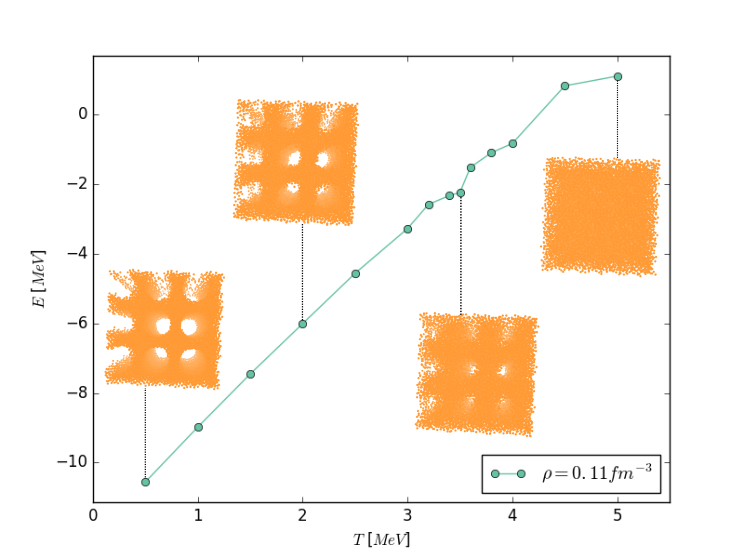
\includegraphics[trim = 5mm 0mm 10mm 5mm, clip, width=0.48\textwidth]{NM/EvsT_tuneles.png}
	\caption{Curvas calóricas para las densidades representando un tipo de pasta particular; ñoquis, spaghettis, lasagna y túneles.
	La formación de todas ellas ocurre para $3\text{MeV}\leq T\leq4\text{MeV}$.}
	\label{fig:EvsT_pastas}
\end{figure}

La totalidad de las curvas calóricas pueden apreciarse en la \textbf{Figura \ref{fig:EvsT_QCNMx0,5}}, donde vemos una cierta convergencia para $T\leq 2$MeV.
Para $T=5$MeV, las energías resultan decrecientes en $\rho$ pero a medida que $T$ desciende alcanzan una región de transición entre $T=3$MeV y $T=4$MeV.
Para $T\leq2$MeV, las curvas parecen converger a una misma pendiente, lo cual coincide en la \textbf{Figura \ref{fig:EvsT_pastas}} con la formación de pastas bien definidas. 

\begin{figure}[H]
	\centering
	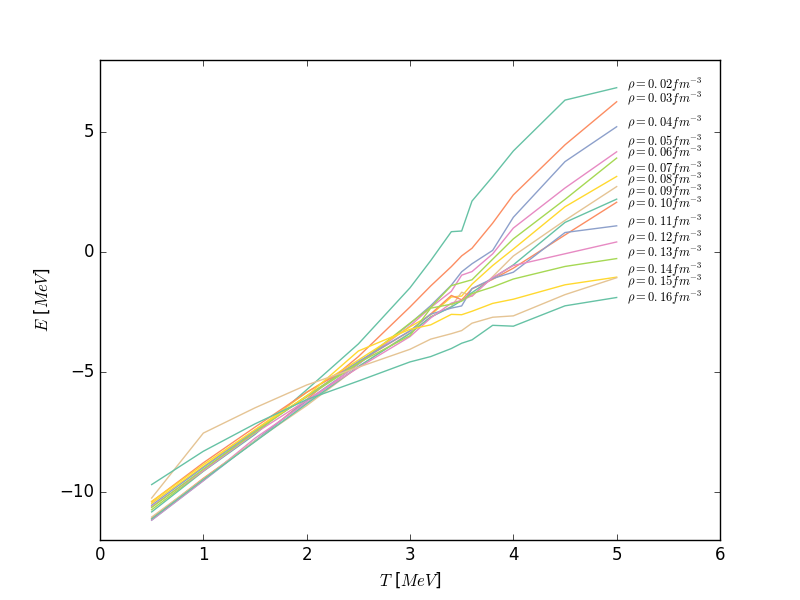
\includegraphics[width=0.9\textwidth]{NM/EvsT_full.png}
	\caption{Curvas calóricas para las distintas densidades. 
	Aunque inicialmente las energías resultan decrecientes en $\rho$, terminan convergiendo para $T\leq 2$MeV.}
	\label{fig:EvsT_QCNMx0,5}
\end{figure}

Este cambio de comportamiento con la temperatura puede apreciarse en la \textbf{Figura \ref{fig:Evsrho_QCNMx0,5}}, donde vemos la curva $E(\rho)$ para  las distintas temperaturas del sistema.
En gris marcamos la región en la que ocurre la aparición de las pastas para la mayor parte de las densidades; correspondiente a $3$MeV$\leq T\leq4$MeV.
Para los valores de $\rho\sim 0.14$fm$^{-3}$ más cercanos a la desaparición de las pastas, esta franja se corre a temperaturas más bajas. 
Es justamente luego de esta transición en $T\sim 3.5$MeV que las curvas $E(\rho)$ pasan de decrecientes a cuasi-constantes, lo cual es más consistente con la existencia de pastas.

Es también llamativo comparando las \textbf{Figuras \ref{fig:Evsrho_QCNMx1}} y \textbf{\ref{fig:Evsrho_QCNMx0,5}} podemos observar que las pastas correspondientes a los distintos rangos de densidades
no parecen verse muy afectados por la reducción de $V_o$. 
La única excepción a esto es la región de burbuja, que al reducir el $V_o$ aumentó a costa de la región de túneles. 
Además, la densidad de transición de pasta a gas se da ahora para $\rho \approx 0.16$fm$^{-3}$, un valor levemente menor al anterior. 
Ciertamente, la forma cóncava de la \textbf{Figura \ref{fig:Evsrho_QCNMx1}} se pierde por completo, por lo que el sistema no parece tener un mínimo claro.
Este mínimo podría encontrarse analizando $\rho\geq 0.16$fm$^{-3}$, pero nos conformamos con que en $T=0.5$MeV las energías para todas las pastas oscilan los $-11$MeV, consistentemente con lo esperado según la \textbf{Figura \ref{fig:curva_Evsrho_dorso}}.

\begin{figure}[H]
	\centering
	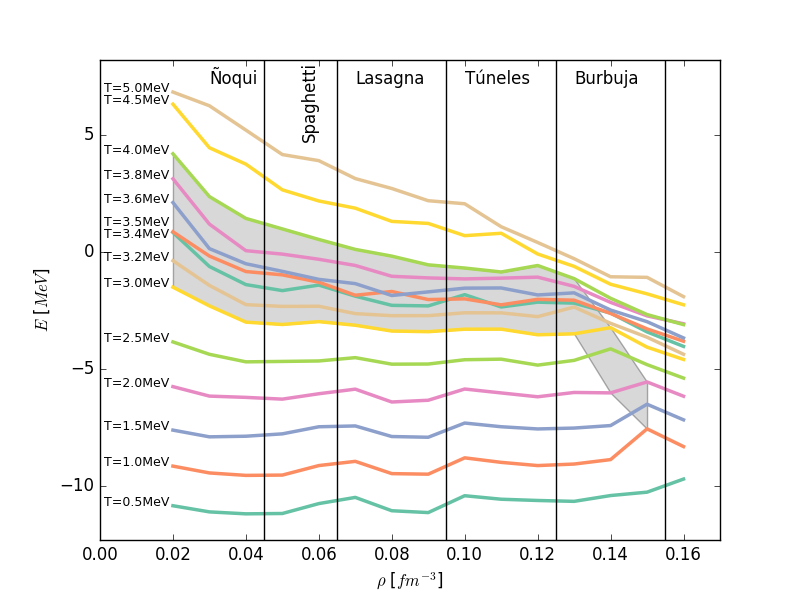
\includegraphics[width=0.9\textwidth]{NM/Evsrho_full.png}
	\caption{Curvas $E$ vs $\rho$ para las distintas temperaturas. 
	La región gris marca el rango de temperaturas en que ocurre la formación de las pastas.
	Es allí también donde se da la transición entre la curva $E$ vs $\rho$ decreciente y la cuasi-constante.
	También se encuentran marcadas con líneas verticales las regiones de densidades correspondientes a cada pasta.}
	\label{fig:Evsrho_QCNMx0,5}
\end{figure}
